%! Author = Vojta
%! Date = 25.11.2021

\chapter{Implementace}
Tato kapitola popisuje tvoření protypu aplikace od založení projektu po vydání první verze. Zmíním zajímavé problémy,
které během implementace nastaly a jak jsem je řešil. Vše staví na předchozích kapitolách, tedy analýze, návrhu a použití
technologií, které jsem představil dříve.

\section{Založení projektu}
Před touto prací jsem neměl žádné zkušenosti se zakládáním větších projektů. Domluvil jsem se tedy s vedoucím a společně
jsme založili projekt pro \emph{Vue} aplikaci. Měl jsem již připravený \emph{Github} repozitář, ve kterém jsem projekt
verzoval~\cite{GithubAbout}.

Pro založení jsem využil \emph{vue ui} (grafická nadstavba \emph{vue cli}), což je grafické rozhraní pro správu \emph{Vue} projektů.
Zde jsem zvolil konfiguraci a přidali pluginy. Poté bylo potřeba některé z nich inicializovat.

\subsection{Firebase}
Nejdříve jsem založili projekt ve \emph{Firebase}. Stačí se přihlásit, otevřít konzoli a kliknout na tlačítko pro vytvoření projektu.
Poté se zadá název, popřípadě se projde konfigurací \emph{Google Analytics}. Rovnou jsem přešel na \emph{Blaze plan}~\cite{FirebasePricing}, díky kterému
se otevřelo více možností. Je ale potřeba si kontrolovat, že aplikace nepřesáhne žádné limity~\cite{FirebaseLimits}, jinak se strhne
částka ze zadané platební karty. To se dá dělat buď manuálně nebo stanovit \emph{budget}, který aplikace nesmí za měsíc přesáhnout.
Po vyčerpání poloviny tohoto limitu přijde upozornění na email správce aplikace~\cite{FirebaseBudget}.

Po založení se do projektu přidá aplikace. Díky tomu \emph{Firebase} vygeneruje kód, který se musí do aplikace přidat.
Pomocí \mintinline{console}|npm install firebase| se do projektu přidá potřebný balíček. Poté je potřeba přidat vygenerovaný
kód. Dále jsem nainstaloval přes \mintinline{console}|npm install -g firebase-tools| \emph{Firebase CLI}. Toto rozhraní umožní
ovládání všech služeb, které \emph{Firebase} nabízí přímo z konzole. Nakonec je nutné se přihlásit (\mintinline{console}|firebase login|) a % TODO: Popsat config?
inicializovat projekt (\mintinline{console}|firebase init|). Při inicializaci je řada možností, vybrat si které služby jsou potřeba,
a které nikoliv. Je také možné nastavit automatický \emph{deploy} při nahrání kódu na \emph{Github}.

\subsection{Automatický deploy}
Je velmi pohodlné, když se při změně kódu automaticky nahraje nová verze i na produkci. Proto jsem tuto funkci nastavil hned
při zakládání projektu a po celou dobu vývoje, jsem měl do pár minut po nahrání dostupnou verzi pro testování odkudkoliv.

Při \mintinline{console}|firebase init| se vytvoří \emph{yml} soubory v složce \emph{.github}. Díky těmto souborům se pak při
\emph{pull requestu} nebo \emph{merge} spustí proces, který sestaví aplikaci a výsledný \emph{build} nahraje na \emph{Firebase Hosting}~\cite{FirebaseHosting}.

\section{Struktura projektu}
Vytvoření složek a základní rozdělení jsem ponechal na \emph{vue ui}. Konfigurační soubory se nachází v \emph{rootu} projektu, implementace
je poté rozdělena podle zaměření ve složce \textbf{src}. Dále se při přidání \emph{Firebase Functions} objevila složka \textbf{functions}, která
obsahuje kód, který se nahrává na server a dá se poté využít jako jednoduché API. Složka \textbf{public} obsahuje základní soubory, jako je \textbf{index.html},
do kterého se při přístupu na stránku vloží JavaScriptový kód nebo různé ikony, jako je logo. Pro výsledný \emph{build}, který se nahraje na Firebase hosting se
používá složka \textbf{dist}.
% TODO: Vložení výpisu?

\begin{figure}
    \dirtree{%
        .1 \\.github\DTcomment{adresář s konfiguračními soubory Githubu}.
        .1 dist\DTcomment{adresář pro sestavenou produkční verzi}.
        .1 functions\DTcomment{adresář s implementaci Firebase Functions}.
        .1 node\_modules\DTcomment{adresář s moduli staženými pomocí Yarn\/npm}.
        .1 public\DTcomment{adresář s obrázky aplikace a základním souborem}.
        .1 src\DTcomment{zdrojové kódy}.
        .2 assets\DTcomment{obrázky využité v aplikaci}.
        .2 components\DTcomment{Vue komponenty}.
        .2 enum.
        .2 lang\DTcomment{překlady}.
        .2 plugins\DTcomment{obaly použitých knihoven}.
        .2 router\DTcomment{adrešář pluginu Vue router}.
        .2 service.
        .2 store\DTcomment{adrešář pluginu Vuex}.
        .2 style\DTcomment{CSS soubory}.
        .2 views\DTcomment{Vue komponenty využívané ve Vue router pro zobrazení stránek}.
        .1 firebase.json\DTcomment{konfigurační soubor Firebase}.
        .1 firebaseConfig.js\DTcomment{tajný konfigurační soubor Firebase}.
        .1 package.json\DTcomment{soubor obsahující seznam závistlostí a konfiguraci aplikace}.
    }
    \caption{Adresářová struktura} \label{fig:struktura}
\end{figure}

\section{Router}
% TODO: Router
Jako první věc jsem si připravil základní cesty aplikace. Cesty se přidávají jako pole objektů, kde objekt obsahuje políčka \emph{path, name, component \emph{a} meta}.
Všechny tyto parametry nejsou povinné a u některých cest jsou i další, které popíšu později. \emph{Path} je string, který následuje za adresou stránky např.
\emph{www.recipeo.cz\textbf{/example}}. \emph{Name} je název dané cesty, který se používá interně v kódu. Tato vlastnost se hodí, když programátor chce změnit adresu stránky.
Díky využití názvu cesty ji nemusí všude v aplikaci přepisovat. \emph{Component} specifikuje komponentu, která se na adrese zobrazí a \emph{meta} jsem zde využit pro změnu
titulku stránky.

Pro některé stránky bylo nutné ověřit, zda je uživatel přihlášený. K tomu lze využít \emph{navigation guards}. Tato ochrana se spustí
vždy před přístupem na stránku a vyhodnotí, zda je požadavek validní. Pokud není, uživatel je přesměrován na jinou stránku.

\begin{listing}[h]
    \caption{Příklad ochrany stránky proti nepřihlášeným uživatelům}
    \begin{minted}{js}
    async function authGuard(to, from, next) {
      if (!await Auth.getCurrentUser()) next({ name: "Login" })
      else {
        next()
      }
    }
    \end{minted}
\end{listing}
\begin{listing}[h]
    \caption{Použití Auth Guardu na stránce profilu uživatele}
    \begin{minted}{js}
    {
        path: "/account",
        name: "Account",
        component: Account,
        meta: { title: "account" },
        beforeEnter: authGuard
    }
    \end{minted}
\end{listing}

Také jsem využil globální úpravy \emph{routeru}, pro aktualizaci názvu stránky. Funguje na stejném principu jako výše zmíněná
ochrana, ovšem provede se na všech stránkách.

\section{Překlady}
Ačkoliv jsme se nakonec s vedoucím rozhodli aplikaci ponechat pouze v čestině, již od začátku jsem ji psal dvojjazyčně a to sice
česky a anglicky. Použil jsem plugin \emph{vue-i18n}. Pro překlady se využívají \emph{.js} soubory, ve kterých se pomocí objektů
strukturují cesty, na které se poté odkazuje ve Vue komponentách.

\begin{listing}[h]
    \caption{Překlad pro recepty}
    \begin{minted}{js}
    recipes: {
      recipes: "Recepty",
      visibility: {
        public: "Veřejný",
        private: "Soukromý",
        unlisted: "Neveřejný"
      },
      noRecipes: "Žádné recepty nenalezeny"
    }
    \end{minted}
\end{listing}

Překlad se vyvolá v \emph{template} pomocí funkce \emph{\$t}, které se jako parametr předá cesta překladu. V \emph{script}
tagu se můžeme na funkci odkazovat přes \emph{this.\$t} a v externích js souborech například přes \emph{i18n.t(recipes)}, kde
\emph{i18n} je naimportovaný ze souboru \emph{router/index.js}.

\begin{listing}[H]
    \caption{Použití překladu}
    \begin{minted}{html}
    <span>{{ $t(recipes.noRecipes) }}</span>
    \end{minted}
\end{listing}

\section{Vuex}
Pomocí Vuex jsem spravoval data přímo v paměti. Vždy po spuštění aplikace se sem nahrála data receptů, ingrediencí, štítků
nebo údaje o uživateli. Pomocí \emph{actions} se volal mnou vytvořený obal pro \emph{Firestore}, odkud se stáhla data buď ze serveru
nebo s lokální cache. Poté se přes \emph{mutations} přidala nová data přímo do Vuexu. Zvolil jsem data, kterých bylo více jednoho typu,
uchovávat v objektech místo obyčejných polí. Získal jsem tím konstantní časovou složitost při přístupu k prvku přes identifikátor. Také
jsem díky tomu nemusel kontrolovat, zda recept s daným \emph{id} existuje, když se stahovala aktualizace. Recept se pouze přepsal novými
daty.

\section{PWA}
Co se týče \emph{PWA}, změnil jsem v konfiguračním souboru název a tématickou barvu. Poté jsem přidat komponentu pro aktualizaci aplikace.
Uživateli se zobrazí, když je na server nahrána nová verze. Uživatel poté klikne na tlačítko \emph{Obnovit} a aplikace se spustí s novou verzí.
Tento dialog se mi nejdříve nedařilo správně zobrazovat, protože jsem posílal špatný typ zprávy pro \emph{service workera}. Místo objektu s
klíčem \emph{type} jsem posílal pouze string se zprávou~\cite{PWAServiceWorker}.

\begin{listing}[h]
    \caption{Správná zpráva pro aktualizaci}
    \begin{minted}{js}
    this.registration.waiting.postMessage({ type: 'SKIP_WAITING' })
    \end{minted}
\end{listing}

\section{Stylování aplikace}
Vzhled aplikace se při vývoji přizpůsobil knihovně Vuetify, ale celkový koncept zůstal zachován. Některé části aplikace
se pročistily a staly se více přehledné. Začínal jsem pouze se světlým režimem, ale v průběhu jsem přidal i tmavý mód.
Bylo potřeba zvolit tmavší pozadí, tak aby bylo podobné tomu původnímu. Vytvořil jsem tedy v aplikaci Illustrator nový projekt
a pustil se do tvoření. Barvy jsem zvolil podle světlého pozadí, ale ztmavil jsem je.

Pro různé režimy jsem odlišil barvy prvků na stránce. Ve světlém jsem se rozhodl pro výrazně modrou \emph{\#1d7dee} \fcolorbox{black}{recipeo-light-blue}{\rule{0pt}{6pt}\rule{6pt}{0pt}} a k tomu
pastelově zelenou \emph{\#79ffa1} \fcolorbox{black}{recipeo-light-green}{\rule{0pt}{6pt}\rule{6pt}{0pt}} , naopak v tmavém jsem použil tlumené odstíny těchto barev a to sice \emph{\#4372b4} \fcolorbox{black}{recipeo-dark-blue}{\rule{0pt}{6pt}\rule{6pt}{0pt}}  a \emph{\#4ca262} \fcolorbox{black}{recipeo-dark-green}{\rule{0pt}{6pt}\rule{6pt}{0pt}} .
Pro změnu barev jsem využil Vuetify a jeho nastavení \emph{theme}. Komponenty z Vuetify mají většinou \emph{prop color}, díky
kterému je možné změnit barvu. Pro prvky mimo Vuetify je možné využít CSS proměnné, která se automaticky vytvoří.

\section{Firebase}

Knihovnu Firebase jsem již představil v předchozích kapitolách. V této sekci popíšu jak knihovnu používat.

\subsection{Firebase Auth}
\emph{Firebase} dokáže řešit i přihlášení uživatele. Nejprve jsem chtěl mít dva způsoby přihlášení, přes email a heslo a přes
Google. Nakonec po domluvě s vedoucím jsem zvolil prozatím ponechat pouze Google přihlášení, abychom nemuseli řešit ukládání
dat uživatele jinam než právě do \emph{Auth}~\cite{FirebaseAuth}. Zapnutí různých možností autentizace je možné ve webové konzoli. V případě Googlu
stačilo přidat kontaktní email a služba se spustila.

Na frontendu jsem tedy vytvořil formulář pro přihlášení a registraci. Pro budoucí využití pří případném přechodu na jinou formu
autentizace se tyto formuláře hodí. Ale v první verzi bude zpřístupněn pouze Google \emph{sign-in provider} a to sice přes \emph{pop-up},
který se uživateli zobrazí při kliknutí na tlačítko přihlášení. Metoda která tuto funkčnost poskytuje se dá naimportovat přímo
z \emph{Firebase}. Musel jsem ale upravit konfigurační soubor, ve které jsem změnil hodnotu \emph{authDomain} na \emph{recipeo.cz}.
Díky tomu se \emph{pop-up} otevře na naší doméně a ne na původní vygenerované.

\subsection{Firestore cache}
% TODO: Jak se fulltext. řešilo s Algolií
\subsubsection{Algolia}
Jak jsem již popisoval, nejdříve jsem zvolil řešení s technologií Algolia. Bylo tedy potřeba založit nový projekt. Po jeho založení
jsem vytvořil index \emph{recipes}, do kterého se synchronizovala data z Firebase. To se dělo díky rozšíření~\cite{AlgoliaExtension}, které vytvořilo přímo
zastoupení Algolie. Měl jsem nejdříve s tímto rozšířením problémy, ale později jsem zjistil, že se mi data nesynchronizují, protože jsem
poskytl do naší aplikace ve Firebase špatný API klíč. Ten měl práva pouze na čtení, ovšem už ne na zápis. Synchronizace se tedy vždy odeslala,
ale Algolia ji odmítnula a ponechala v indexu stará data.

Po prvních pár dnech jsem zjistil, že počet čtení je celkem vysoký, hlavně kvůli tomu, že se vyhledávání na serveru spustí po
každém napsaném písmenku. Využil jsem tedy \emph{debounce} funkci, která tato vyhledávání snížila. \emph{Debounce} funguje tak,
že se spustí vždy, když uživatel stiskne klávesu na klávesnici. Poté je nastavený časový limit a pokud do té doby nic nenapíše,
spustí se \emph{callback}, tedy v našem případě funkce která zařídí vyhledávání.

Dále jsem díky~\cite{AlgoliaBlog} zjistil, že je možné limitovat volání při načtení komponenty. V základu se totiž při každém
načtení vyčerpají dvě zavolání kvůli optimalizaci rychlosti vyhledávání.

I přes všechny tyto vylepšení bylo nemožné udržet počet vyhledávání pod limitem 10 000 za měsíc, protože já samotný při vývoji,
kdy jsem až tolik vyhledávání nevyužíval, vyčerpal přes deset procent z limitu.

\subsubsection{Cache}
K implementaci cache jsem přistoupil, když bylo jasné, že Algolia je nepoužitelná. Musel jsem tedy vymyslet jiný způsob fulltextového
vyhledávání a jako nejlepší způsob se nabízelo stáhnou všechna potřebná data a filtr aplikovat přímo na zařízení uživatele. To je ale
spojeno s nákladnými operacemi nad databází při každém spuštění aplikace, a proto bylo nutné implementovat cache.

Základní spuštění je velmi jednoduché, stačí zavolat importovanou metodu z Firebase.

\begin{listing}[h]
    \caption{Zapnutí perzistentního módu}
    \begin{minted}{js}
    enableIndexedDbPersistence(db, {forceOwnership: true} )
    .catch((err) => {
        if (err.code === "failed-precondition") {
            console.log("Multiple tabs open, persistence can only be enabled
            in one tab at a a time.")
        } else if (err.code === "unimplemented") {
            console.log("The current browser does not support all of the
            features required to enable persistence")
        }
    })
    \end{minted}
\end{listing}

Jako parametr je potřeba předat instanci Firestore, kterou lze získat s parametrem pro neomezenou velikost, tím pádem se nebudou
mazat záznamy kvůli úspoře místa. Je také nutné přidat parametr \emph{forceOwnership}, protože jinak se cache rozbije při více
otevřených záložkách se stejnou aplikací~\cite{FirebaseMultipleTabs}.

\begin{listing}[h]
    \caption{Získání instance Firestore}
    \begin{minted}{js}
    const db = initializeFirestore(FirebaseApp, {
        cacheSizeBytes: CACHE_SIZE_UNLIMITED
    })
    \end{minted}
\end{listing}
% TODO: Navázat na sekci z designu

Poté jsem vytvořil funkci, která se starala o to, odkud se mají data stahovat. Při každém stažení jsem si v \emph{local storage} aktualizoval
časovou značku a díky tomu jsem mohl stahovat pouze data, se kterými mezitím bylo manipulováno. Zde se objevilo několik problémů. Jeden z nich
bylo to, že jakmile se přihlásil jeden uživatel, poté se ihned odhlásil a přihlásil se jiný, recepty se nestáhnuly správně. Bylo proto potřeba
aktualizovat časovou značku při každé manipulaci s autorizací.

\begin{listing}[H]
    \caption{Metoda pro stažení dat}
    \begin{minted}{js}
    async getData () {
      if(!lastUpdated || !expirationDate) {
        // Download everything from server and add timestamps to localStorage.
        addTimestamps()
        Store.dispatch("getData", { source: FirestoreSource.SERVER, updateOnly: false })
        return
      }

      if(Date.now() > expirationDate) {
        // Download everything from server and add timestamps to localStorage.
        addTimestamps()
        Store.dispatch("getData", { source: FirestoreSource.SERVER, updateOnly: false })
      }
      else {
        // Get data from cache, call query to update new data and set last updated timestamp.
        localStorage.lastUpdated = Date.now()
        await Store.dispatch("getData", { source: FirestoreSource.CACHE, updateOnly: false })
        await Store.dispatch("getData", { source: FirestoreSource.SERVER, updateOnly: true })
      }
    }
    \end{minted}
\end{listing}


\subsection{Firestore rules}
Bezpečnost je důležitá součást jakéhokoliv softwaru. Firebase proto nabízí takzvané Firestore Rules pro zabezpečení dat na serveru.
Díky těmto pravidlům je možné filtrovat požadavky a v případě nutnosti zamítnout přístup k datům. Zvolil jsem pravidla na základě
indentifikace pomocí \emph{uid} neboli uživatelského identifikátoru. Pravidla fungují tak, že se pomocí cesty ve Firestore vyhledá
pravidlo a pokud je splněna podmínka, data se odešlou. Ve výchozím stavu jsou všechny zdroje privátní, tedy nikdo v nim nemá přístup.

\begin{listing}[H]
    \caption{Pravidlo pro přístup k veřejnému receptu}
    \begin{minted}{js}
    match /{path=**}/recipes/{doc} {
        allow read: if resource.data.visibility == "public";
    }
    \end{minted}
\end{listing}

Při zobrazení editace pravidel se v levé části pod historií pravidel nachází \emph{Rules playground}~\cite{FirebaseRulesPlayground}. V této záložce je možné
testovat vytvořená pravidla. Vývojář může zvolit typ dotazu, tedy \emph{get, create, update \emph{nebo} delete}, dále specifikovat
zdroj, ze kterého chceme data dostat (nějaká kolekce) a nakonec určit, zda se požadavek bude simulován pod přihlášeným uživatelem
či nikoliv. U uživatele lze nastavit \emph{provider}, \emph{uid}, email (i zda byl verifikován), jméno a telefon. Nakonec se pomocí tlačítka
\emph{run} dotaz spustí a v pravé části u pravidel se graficky zobrazí, kde byl přístup povolen a kde odmítnut.


\begin{figure}[H]
    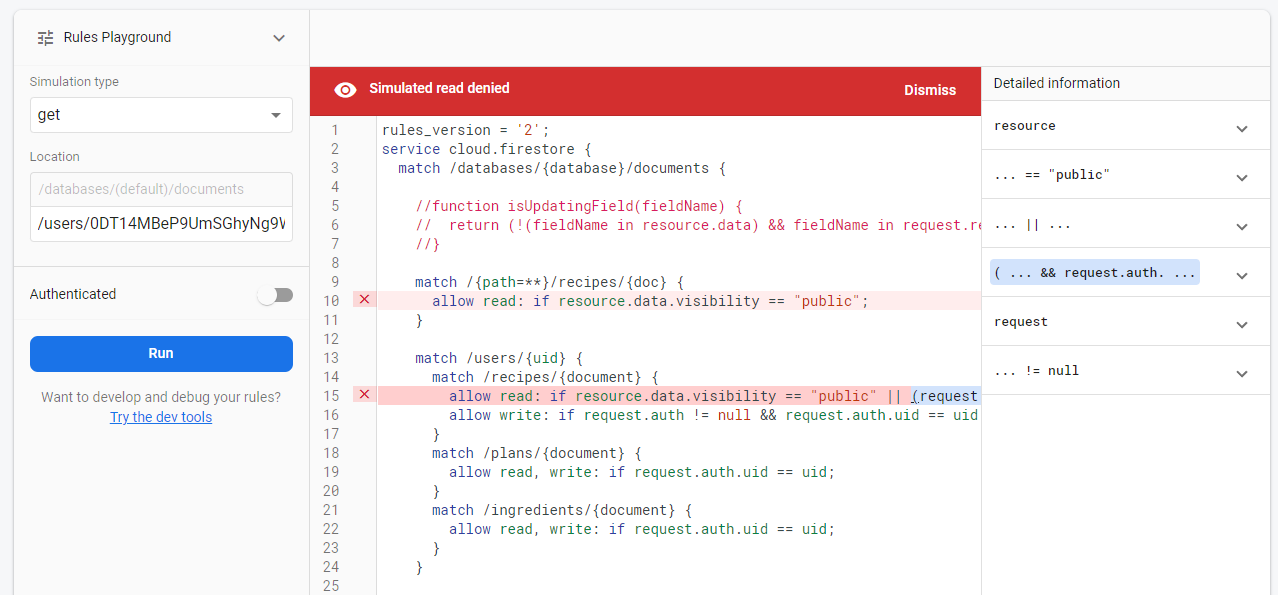
\includegraphics[width=\textwidth]{images/recipeo-rules-denied}
    \caption{Zablokování přístupu v Rules playground} \label{picture:recipeo:rules-denied}
\end{figure}

\begin{figure}[H]
    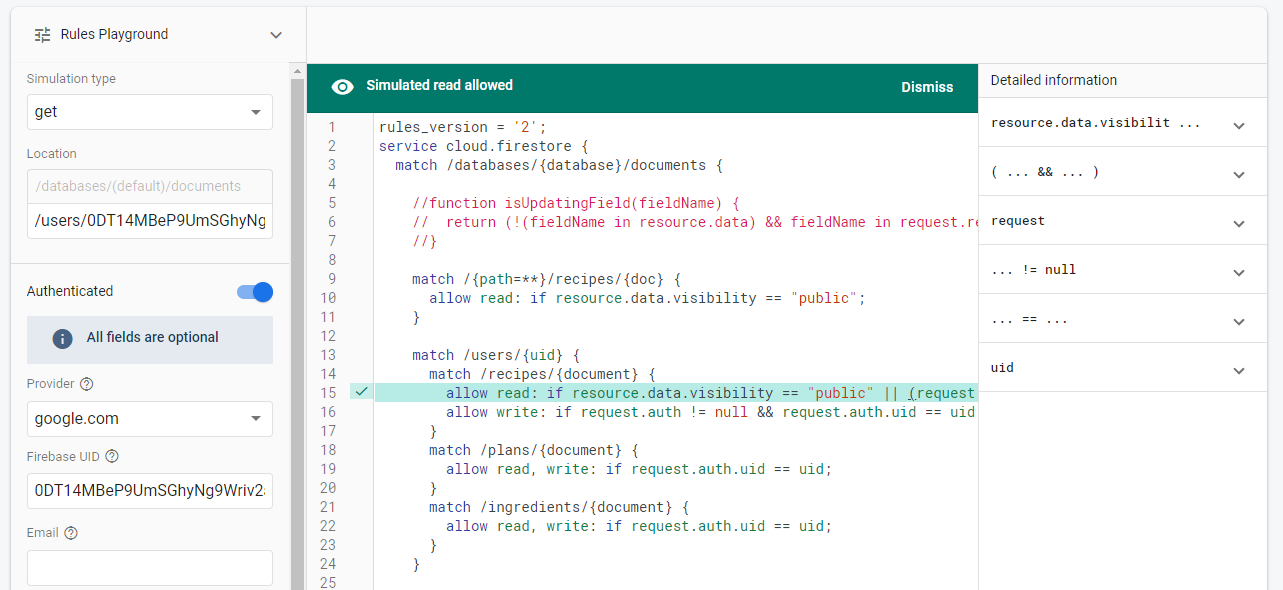
\includegraphics[width=\textwidth]{images/recipeo-rules-allowed}
    \caption{Povolení přístupu v Rules playground} \label{picture:recipeo:rules-allowed}
\end{figure}

\subsection{Firebase Functions}
Cloudové funkce~\cite{FirebaseFunctions} jsem využil pro místa v aplikaci, kde nebylo možné pomocí Firestore Rules správně ošetřit bezpečnost dat.
Poprvé jsem napsal funkce, díky kterým se stáhnul určitý počet receptů, ke kterým měl uživatel přístup. Využil jsem stránkování,
což znamená, že když uživatel přišel na stránku s recepty, stáhlo se pouze omezené množství a až když bylo potřeba, aplikace požádala
server o další. Díky tomu jsem nemusel vytvářet žádná pravidla, stačilo nechat celou databázi zamknutou, protože ve Functions se přistupuje
k datům přes admin účet, který má práva na veškeré operace. Nakonec toho ale nebyl vhodný přístup, a tak jsem funkce odstranil.

Kde se tento přístup hodil bylo u pozvánek do skupiny. Pozvanému uživateli se musí zobrazit informace o skupině, ten ale ještě ve skupině není,
a tak nemá k těmto datům přístup. Proto se zavolá z aplikace funkce \emph{getGroup}, která odešle zpátky záznam dané skupiny. Poté se uživateli
zobrazí dialog s pozvánkou a tlačítko \emph{Připojit}. Po stisku tohoto tlačítka se opět zavolá jedna z funkcí, tentokrát \emph{joinGroup}. Ta
zapíše identifikátor uživatele do pole \emph{userIds}, které je v dokumentu dané skupiny. K tomu se dá využít funkce \emph{arrayUnion}, kterou poskytuje
Firebase k jednoduchým operacím na poli. Díky tomu se nemůže stát, že by nastala duplikace jednoho uživatele.

Firebase nabízí různé typy emulátorů, ovšem jediný který jsem využil byl právě \emph{Functions emulator}~\cite{FirebaseEmulator}. Díky tomu jsem mohl lokálně testovat, jak vypadají
data, která odesílá server a nemusel pokaždé čekat, než se funkce nahrají na server, což při větším počtu trvá až několik minut. Také jsem tento lokální server
využil při problémech s právy. Několikrát se mi stalo, že funkce spadla či mi odepřela přístup. Pomocí emulátoru jsem tak zjistil, zda je špatně napsaná funkce
nebo není správně nakonfigurovaná. Poté jsem našel v dokumentaci našel, že je potřeba u některých funkcí přidat roli pro autorizování volání funkce v Google
Cloud platfomě~\cite{CloudRights}.

% TODO: Problémy s přístupem k funkci https://console.cloud.google.com/functions/details/europe-west3/joinGroup?project=recipeo-2e1c9&authuser=0&hl=en&tab=permissions

% TODO: Stylování aplikace a Vuetify
